\subsection{ViT-B\slash{}16}

\paragraph{Entrenamiento desde cero (scratch + normalizado):}
ViT-B/16, el modelo con mayor capacidad del estudio (85.8M de parámetros), fue entrenado desde cero con el pipeline de normalización estricta durante 30 épocas con tasa de aprendizaje fija de $1\times10^{-4}$. Las métricas obtenidas se presentan en la Tabla~\ref{tab:vit_scratch_metrics}.

\begin{table}[H]
\centering
\caption{Métricas de ViT-B\slash{}16 entrenado desde cero con pipeline normalizado.}
\label{tab:vit_scratch_metrics}
\begin{tabular}{lc}
\hline
Métrica & Valor \\
\hline
Accuracy  & 95.74\% \\
Balanced Accuracy & 95.53\% \\
Precisión & 97.38\% \\
Recall (Sensibilidad) & 95.84\% \\
Especificidad & 95.22\% \\
F1-Score & 96.61\% \\
MCC & 0.8916 \\
AUC-ROC & 0.9892 \\
\hline
\end{tabular}
\end{table}

ViT-B/16 obtuvo el accuracy más bajo del estudio (95.74\%), a pesar de triplicar en parámetros a Swin-T y tener 21 veces más parámetros que EfficientNet-B0. La ausencia de sesgos inductivos convolucionales obliga al modelo a aprender desde cero todas las relaciones espaciales, lo que resulta ineficiente con un dataset de solo 6893 imágenes. El entrenamiento, sin embargo, fue saludable: las curvas de aprendizaje (Figura~\ref{fig:vit_scratch_lc}) muestran convergencia paralela entre train y validación, sin la divergencia característica del sobreajuste observado en configuraciones con transfer learning.

\begin{figure}[H]
\centering
    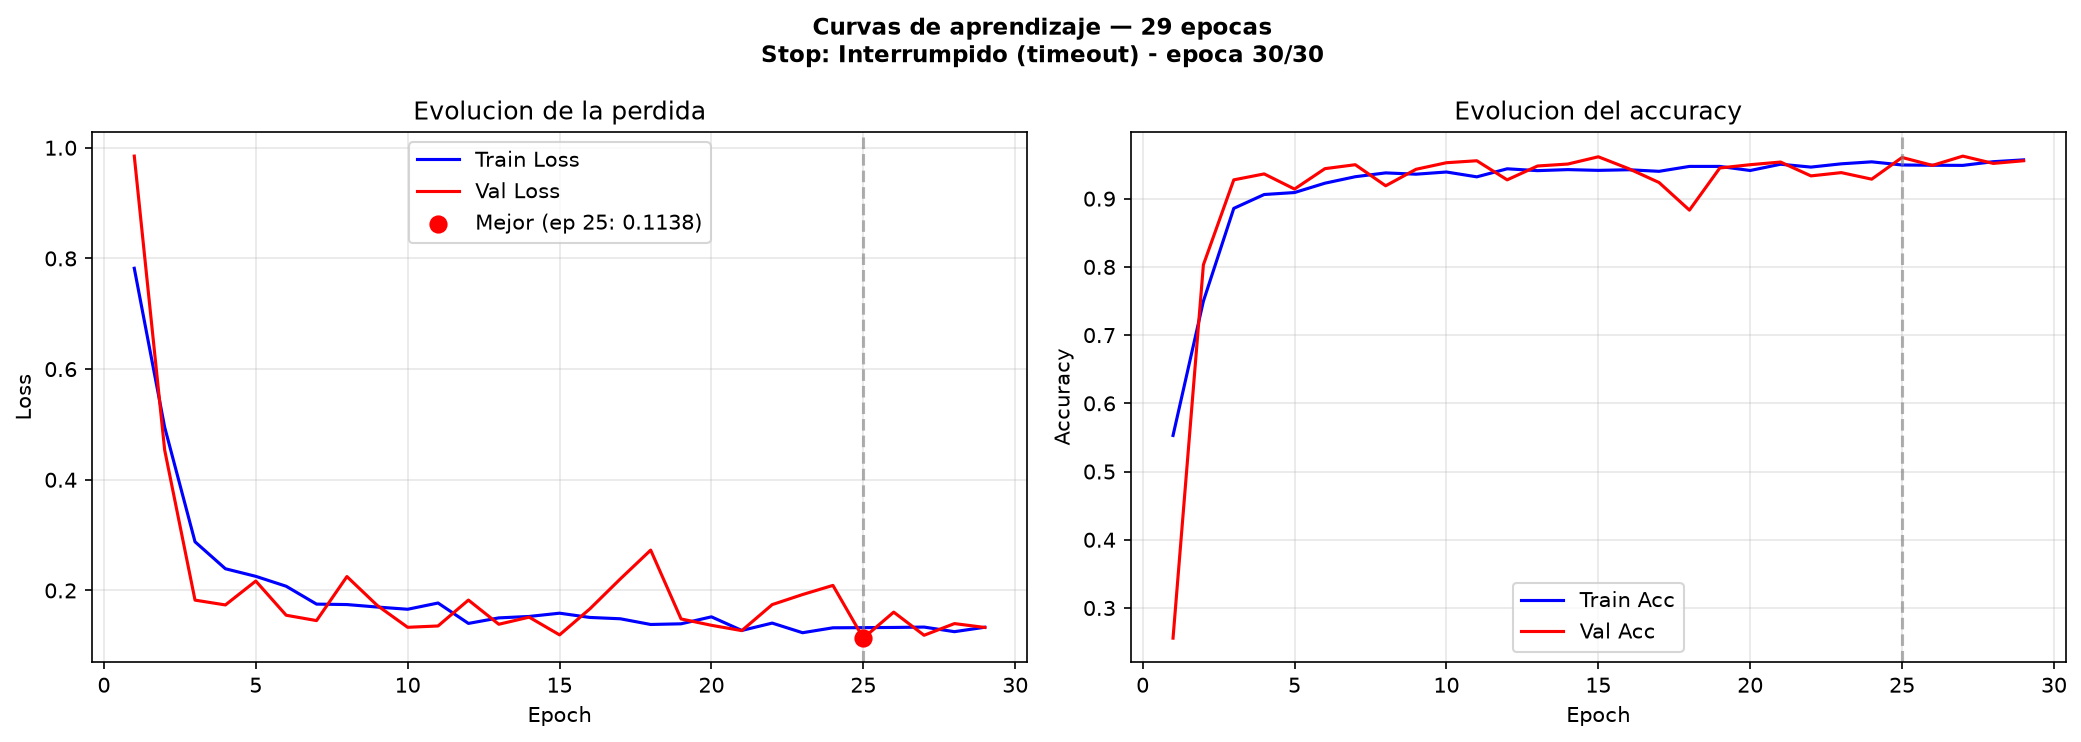
\includegraphics[width=0.95\columnwidth]{../BrainTumor/results/vit/normalized_scratch/learning_curves.png}
    \caption{Curvas de aprendizaje de ViT-B\slash{}16 desde cero con pipeline normalizado.}
    \label{fig:vit_scratch_lc}
\end{figure}
